\documentclass[]{beamer}

\usetheme{Rochester}
\usecolortheme{dove}
\setbeamercolor{section in head/foot}{fg=white, bg=black}
\setbeamertemplate{title page}[default][colsep=-4bp,rounded=true]
\usefonttheme{serif}

\usepackage{newpxtext}
\usepackage{newpxmath}
\usepackage{amsmath}
\usepackage{amssymb}
\usepackage{amsthm}
\usepackage{bbm}
\usepackage{graphicx}
\usepackage{multicol}
\usepackage{animate}

\title[MAT 336 Final Project]{Algorithm Benchmarking Analysis}
\author{Vasilisa Bashlovkina, David Kraemer, Bo Wang}
\date{May 9 2016}

\renewcommand{\emph}{\textbf}
\newcommand{\N}{\mathbbm{N}}
\newcommand{\R}{\mathbbm{R}}
\newcommand{\Order}{\mathcal{O}}
\DeclareMathOperator*{\uniform}{\mathsf{Uniform}}



\begin{document}

\begin{frame}
\titlepage
\end{frame}

\section{Introduction}


\begin{frame}[t]{Introduction}

\begin{itemize}
	\item An algorithm's ``worst-case'' run-time is a useful object of study in computer science.
    \item Denote $f : \N \to \N$ where for a given input $n$, $f(n)$ is the steps required for the algorithm to terminate.
    \begin{definition}
	We say a function $f$ has \emph{order $g$} and write $f(n) \in \Order(g(n))$ if there exist $c \in \R$ and $N \in \N$ such that
    \[
    f(n) \leq c \cdot g(n)
    \]
    for all $n \geq N$. 
	\end{definition}
    \item This is called \emph{Big-Oh} analysis.
\end{itemize}
\end{frame}

\begin{frame}[t]{Sorting}
\begin{block}{Problem}
Given an array $A$, rearrange elements of $A$ such that $A[k] \leq A[k+1]$ for all $k$.
\end{block}
\begin{itemize}
	\item We consider two algorithms: \emph{insertion sort} and \emph{merge sort}.
    \item Insertion sort has worst-case complexity $\Order(n^2)$.
    \item Merge sort has worst-case complexity $\Order(n \log_2 n)$.
    \item In theory, merge sort is \emph{much} faster than insertion sort.
\end{itemize}
\end{frame}

\begin{frame}[t]{Insertion sort}
    \centering
    \animategraphics[autoplay, height=5cm]{24}{insert/insert-}{0}{454} 
    \footnote{Attribution: \url{http://www.sorting-algorithms.com/insertion-sort}}
\end{frame}

\begin{frame}[t]{Merge sort}
    \centering
    \animategraphics[loop,autoplay]{24}{merge/merge-sort-}{0}{217} 
    \footnote{Attribution: \url{http://www.sorting-algorithms.com/merge-sort}}
\end{frame}

\begin{frame}[t]{Search}
\begin{block}{Problem}
Given a sorted array $A$ and entry $v$, determine the index $k$ such that $A[k] = v$.
\end{block}
\begin{itemize}
	\item We consider two algorithms: \emph{linear search} and \emph{binary search}.
    \item Linear search has worst-case complexity $\Order(n)$.
    \item Binary search has worst-case complexity $\Order(\log_2 n)$.
    \item In theory, binary search is \emph{much} faster than linear search.
\end{itemize}
\end{frame}

\begin{frame}[t]{Binary and linear search}
    \centering
    \animategraphics[loop,autoplay,height=5cm]{18}{search/search-}{0}{220} 
    \footnote{Attribution: \url{http://mrmonline.org/site/binary-search-algorithm/}}
\end{frame}

\begin{frame}[t]{Iteration and recursion}
\begin{itemize}
	\item Algorithms can usually have both iterative and recursive implementations.
    \item The dominant view is that iteration is faster than recursion.
    \item This is due to language-implementation details.
\end{itemize}
\end{frame}


\section{Analysis}
\begin{frame}[t]{Experiments}
	\begin{itemize}
    \item Each algorithm is implemented recursively and iteratively in C, recursively in Scheme, and iteratively in Python.
    \item It is a common perception that C is faster than both Scheme and Python.
    \item We generate arrays of length $n = 1000, \ldots 50000$.
    \item For sorting, the elements are iid $\uniform(0, n)$
    \item For searching, the differences between adjacent elements are iid $\uniform(0,10)$.
	\item We measure program execution time, a rough proxy for steps to termination.
\end{itemize}
\end{frame}

\begin{frame}[t]{Research Questions}
\begin{itemize}
	\item Does the theorized relationship between input and run-time manifest in practice?
    \item Is merge sort empirically faster than insertion sort?
    \item Is binary search empirically faster than linear search?
    \item Is iteration faster than recursion?
    \item Is C faster than Scheme or Python?
    \item What is the relationship between Scheme and Python?
\end{itemize}

\end{frame}

\section{Results and Conclusions}

\begin{frame}{Comparing languages}
\begin{center}
	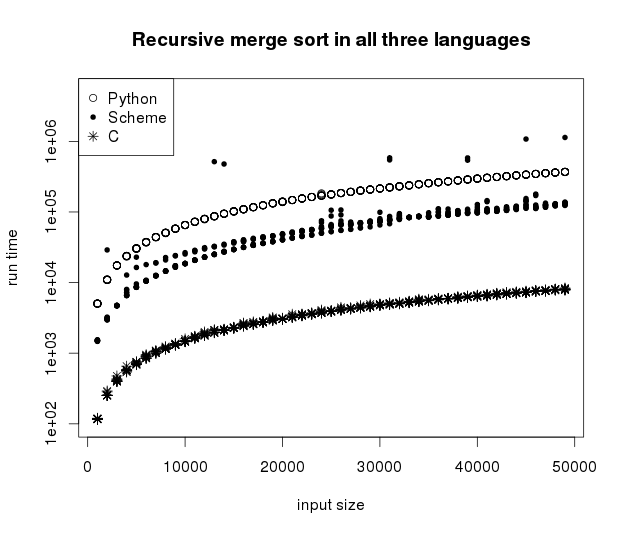
\includegraphics[width=0.8\textwidth]{plots/recursive_merge_in_all_three_lgs.png}
\end{center}
\end{frame}

\begin{frame}[t]{Comparing languages}
\begin{center}
	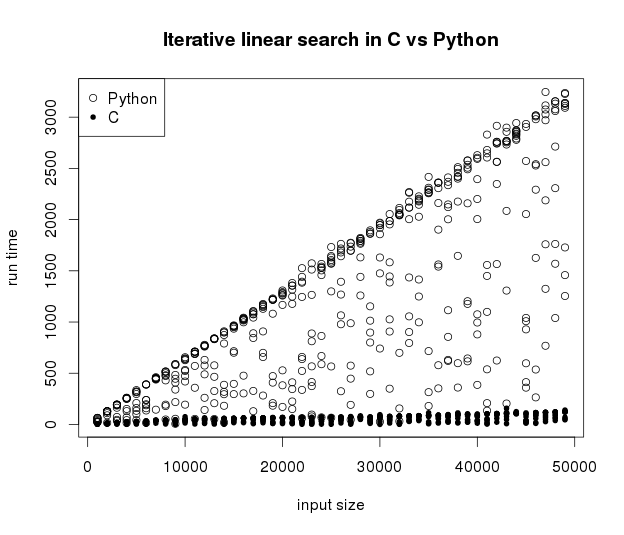
\includegraphics[width=0.8\textwidth]{plots/i_linear_in_c_vs_python.png}
\end{center}
\end{frame}

\begin{frame}[t]{Comparing iteration and recursion}
\begin{center}
	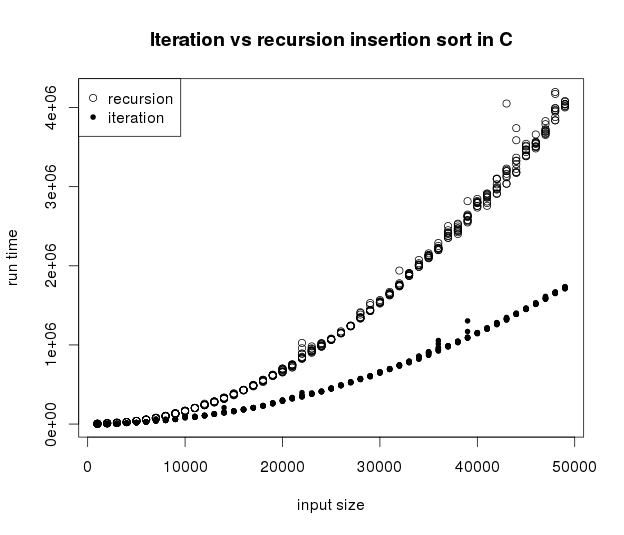
\includegraphics[width=0.8\textwidth]{plots/i_vs_r_insertion_in_c.png}
\end{center}
\end{frame}

\begin{frame}[t]{Comparing sorting algorithms}
\begin{center}
	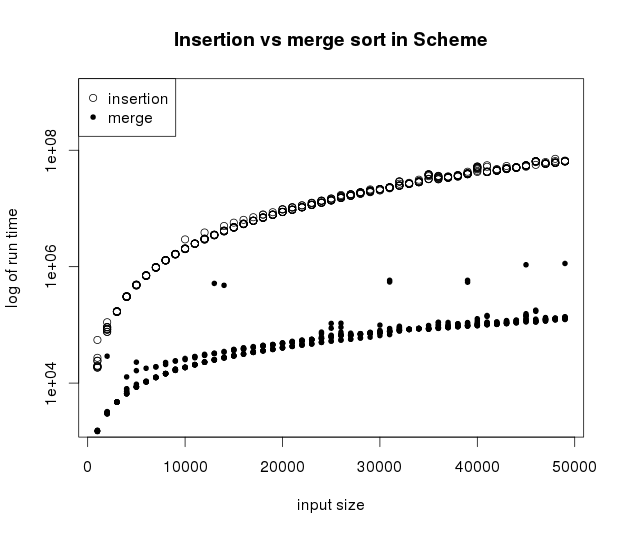
\includegraphics[width=0.8\textwidth]{plots/insertion_vs_merge_in_scheme.png}
\end{center}
\end{frame}

\begin{frame}[t]{Fitted theoretical model}
\begin{center}
	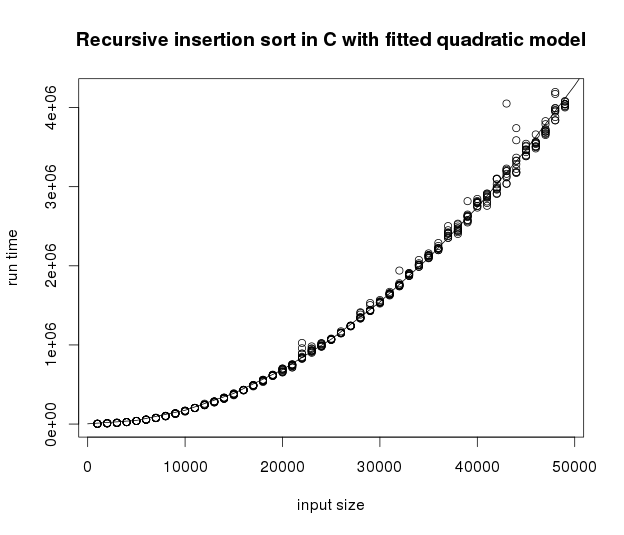
\includegraphics[width=0.8\textwidth]{plots/r-quadratic-regression.png}
\end{center}
\end{frame}

\begin{frame}[t]{Fitted theoretical model}
\begin{center}
	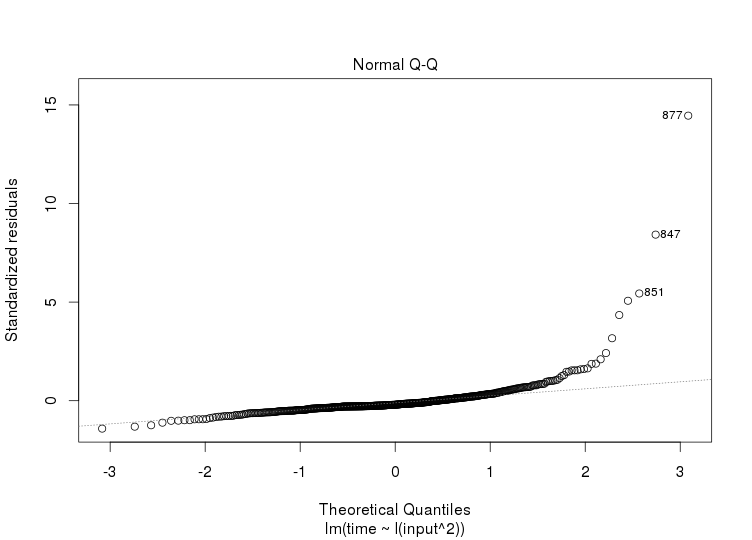
\includegraphics[width=0.8\textwidth]{plots/qq-plot.png}
\end{center}
\end{frame}

\begin{frame}[t]{Methodology and Results}
\begin{itemize}
	\item We used paired $t$-tests to identify significant speed differences between
    \begin{itemize}
		\item recursion vs iteration
        \item C, Scheme, and Python,
        \item linear vs binary search; insertion vs merge sort
\end{itemize}
	\item We found significant ($p < 0.001$) speed differences in almost every comparison.
    \item We found no significant speed difference between recursive and iterative binary search in C ($p = 0.24$).
\end{itemize}
\end{frame}

\begin{frame}[t]{Methodology and Results}
\begin{itemize}
    \item We used transformed linear models to determine if empirical data supports theoretical upper bounds of performance
    \item We found that the theoretical models better fit the data in almost every case.
    \item We did not find this for binary search in C.
\end{itemize}
\end{frame}

\begin{frame}[t]{Conclusion}
\begin{itemize}
	\item The overwhelming evidence is that C is the fastest language, iterative is the fastest paradigm, and merge sort and binary search are the fastest algorithms
    \item We found no significant results for binary search in C because its run time is sub-microsecond.
    \item Should every program be written in C?
    \item Should every algorithm be implemented iteratively?
\end{itemize}
\end{frame}

\end{document}
